\documentclass{minimal}

% Tikz
\usepackage{pgf}
\usepackage{tikz}

\usetikzlibrary{calc,trees,positioning,arrows,chains,shapes.geometric,%
    decorations.pathreplacing,decorations.pathmorphing,shapes,%
    matrix,shapes.symbols,positioning}

\tikzset{
kiste/.style={
    rectangle, 
    rounded corners, 
    % fill=black!10,
    draw=black, very thick,
    text width=10em, 
    minimum height=3em, 
    text centered},
kkiste/.style={
    rectangle, 
    rounded corners, 
    % fill=black!10,
    draw=black, very thick,
    text width=7em, 
    minimum height=2em, 
    text centered},
}

\begin{document}
\begin{center}
 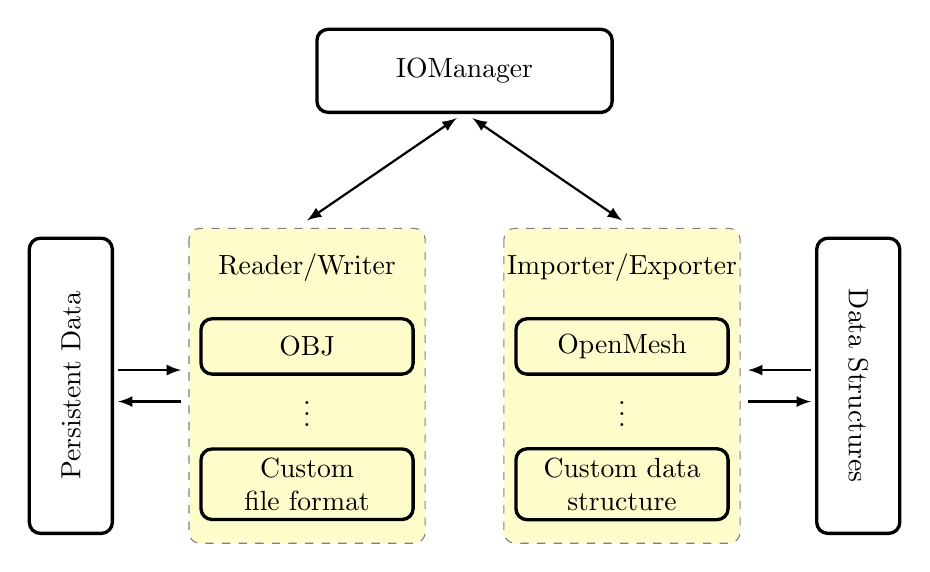
\begin{tikzpicture}
 
\node[kiste](IOM) at (0,0) {IOManager};
\node[kiste,rotate=90](PD) at (-5,-4) {Persistent Data};
\node[kiste,rotate=-90](DS) at (5,-4) {Data Structures};

\path[fill=yellow!20,rounded corners,draw=black!50, dashed]
     (-3.5,-2) rectangle (-0.5,-6);
\path[fill=yellow!20,rounded corners,draw=black!50, dashed]
     (.5,-2) rectangle (3.5,-6);

\node[] at (-2,-2.5) {Reader/Writer};
\node[kkiste] at (-2,-3.5) {OBJ};
\node[] at (-2,-4.25) {$\vdots$};
\node[kkiste] at (-2,-5.25) {Custom file format};

\node[] at (2,-2.5) {Importer/Exporter};
\node[kkiste] at (2,-3.5) {OpenMesh};
\node[] at (2,-4.25) {$\vdots$};
\node[kkiste] at (2,-5.25) {Custom data structure};

\path [draw,thick,>=latex,<->] (-0.1,-0.6) -- (-2,-1.9) {};
\path [draw,thick,>=latex,<->] (0.1,-0.6) -- (2,-1.9) {};

\path [draw,thick,>=latex,->] (-4.4,-3.8) -- (-3.6,-3.8) {};
\path [draw,thick,>=latex,<-] (-4.4,-4.2) -- (-3.6,-4.2) {};

\path [draw,thick,>=latex,->] (4.4,-3.8) -- (3.6,-3.8) {};
\path [draw,thick,>=latex,<-] (4.4,-4.2) -- (3.6,-4.2) {};

\end{tikzpicture}
\end{center}

\end{document}
